\section{Dataset Description}
\label{sec:dataset}

The study uses three public datasets of plane-geometry diagrams and one generated source (Table~\ref{tab:datasets}). The problem places five requirements on the data: real textbook diagrams; the coordinates of every annotated point, so that relations can be measured rather than assumed; human relation annotations, so that the measured truth can be compared with the marked one; a source independent of the training data; and a public licence. Together the four sources meet them: Geometry3K supplies the formal relation language with point positions, PGDP5K accurate positions and a mark-based annotation for the same figures plus a clean unseen source, PGPS9K a large pool of real diagrams, and the synthetic source the verifier-labelled data that \Hone{} is about. Geometry3K's two known defects, noisy coordinates and a problem-level split, are corrected in the pipeline (Section~\ref{sec:preprocessing}).

\begin{table}[tbp]
  \centering\small
  \caption{Data sources. Figure counts are after duplicate-image clustering (Section~\ref{sec:preprocessing}).}
  \label{tab:datasets}
  \begin{tabularx}{\textwidth}{@{}>{\hsize=.6\hsize}Y >{\hsize=1.0\hsize}Y >{\hsize=1.05\hsize}Y >{\hsize=.7\hsize}Y >{\hsize=1.65\hsize}Y@{}}
    \toprule
    Source & Size & Annotation & Coordinates & Role \\
    \midrule
    Geometry3K \cite{lu2021intergps} & \nGeometryProblems{} problems; \nGeometryFigures{} figures & formal language (91 predicates) & yes; offset, noisy & training, validation and in-distribution test \\
    PGDP5K \cite{zhang2022pgdp} & \nPgdpDiagrams{} diagrams & primitives, symbols, text, relation graph & yes; pixel-accurate & cleaner coordinates for shared figures; \nHeldoutFigures{} test figures as the unseen source \\
    PGPS9K \cite{zhang2023pgps} & \nPgpsDiagrams{} diagrams & textual clauses, solution programs & yes & pool of real diagrams used without labels (self-training) \\
    Synthetic & unlimited (\synthPoolMax{} generated) & verifier labels; injected constructions as marks & exact & verifier-labelled training data; extrapolation test \\
    \bottomrule
  \end{tabularx}
\end{table}

\subsection{Geometry3K}

Geometry3K \cite{lu2021intergps} contains \nGeometryProblems{} SAT-style problems, each with a diagram image, the problem text and a formal-language annotation. For the diagram, the annotation gives named points with positions (\texttt{point\_positions}), segments as pairs of point names (\texttt{line\_instances}), circles by their centre point, and relations as logic forms: \texttt{Parallel(Line(A,B), Line(C,D))}, \texttt{Perpendicular}, \texttt{Equals} of two \texttt{LengthOf} terms, \texttt{PointLiesOnCircle} and \texttt{PointLiesOnLine}. The published split is by problem (\nGeometryTrainProblems{} / \nGeometryValProblems{} / \nGeometryTestProblems); the \nGeometryProblems{} problems use only \nGeometryFigures{} distinct figures. The images are PNG with a transparent background, accompanied by a copy in which every annotated point is drawn as a red dot. Three defects matter for this study. The coordinates are not image pixels but carry a per-diagram translation, which the pipeline recovers from the red-dot image. Against PGDP5K's pixel re-annotation of the same images (\nCoordPairs{} image pairs) the median point error is \medianCoordErrorPx{} px, but \pctCoordPairsOverTen\% of the pairs have at least one point more than 10 px off. And \nGeometryTestDupTrain{} of the \nGeometryTestImages{} test images (\pctGeometryTestDupTrain\%) are exact copies of a training image, while \nGeometryTestShareFigure{} (\pctGeometryTestShareFigure\%) share a figure with the training or validation split.

\subsection{PGDP5K}

PGDP5K \cite{zhang2022pgdp} contains \nPgdpDiagrams{} diagrams (\nPgdpTrain{} / \nPgdpVal{} / \nPgdpTest), of which 1,813 are Geometry3K images re-annotated and the rest come from textbooks. The annotation is at the level of primitives in pixel coordinates (points, the longest segment of each line, circles with centre and radius), symbols with a class (perpendicular mark, one to four tick bars, one to three parallel arrows, angle arcs, text) and a relation graph linking symbols to primitives and points to the lines and circles they lie on. Asserted relations are read from the marks: a right-angle symbol asserts \rel{perpendicular} between its two lines, tick marks of the same class assert \rel{equal\_length}, parallel arrows of the same class assert \rel{parallel}, and the incidence relations give \rel{on\_circle} and \rel{collinear}. No tangent is marked anywhere in the three real datasets: \nTangentAssertedAll{} assertion exists in total. The \nHeldoutFigures{} PGDP5K test figures with no Geometry3K copy form the \emph{held-out source}.

\subsection{PGPS9K}

PGPS9K \cite{zhang2023pgps} contains \nPgpsDiagrams{} diagrams in the same primitive format as PGDP5K, paired with 9,022 problems; 1,738 of its diagrams are Geometry3K images, and it also contains \nPgpsImagesGeometryTest{} Geometry3K test images and \nPgpsImagesPgdpTest{} PGDP5K test images, so it can only serve as an unlabelled pool after those copies are removed. Its labels are not used for training; they are unsealed only post hoc to measure pseudo-label precision (Section~\ref{sec:evaluation}).

\subsection{Synthetic diagrams}

Because the verifier can label any diagram whose coordinates are known, generated diagrams provide unlimited training labels, can be made larger than any real diagram, and can contain relations that are rare in textbooks. The generator (Section~\ref{sec:preprocessing}) produces a training pool of \synthPoolMax{} diagrams with \synthPointsMin--\synthPointsMax{} points, of which the first 1,000 and 10,000 are nested subsets for the scaling contrast; an extrapolation pool of \synthExtrapSize{} diagrams with \synthExtrapPointsMin--\synthExtrapPointsMax{} points; and an unlabelled pool of \synthUnlabelledSize{} diagrams whose coordinates are sealed. Fig.~\ref{fig:examples} shows real and synthetic examples with their query overlays.

\begin{figure}[tbp]
  \centering
  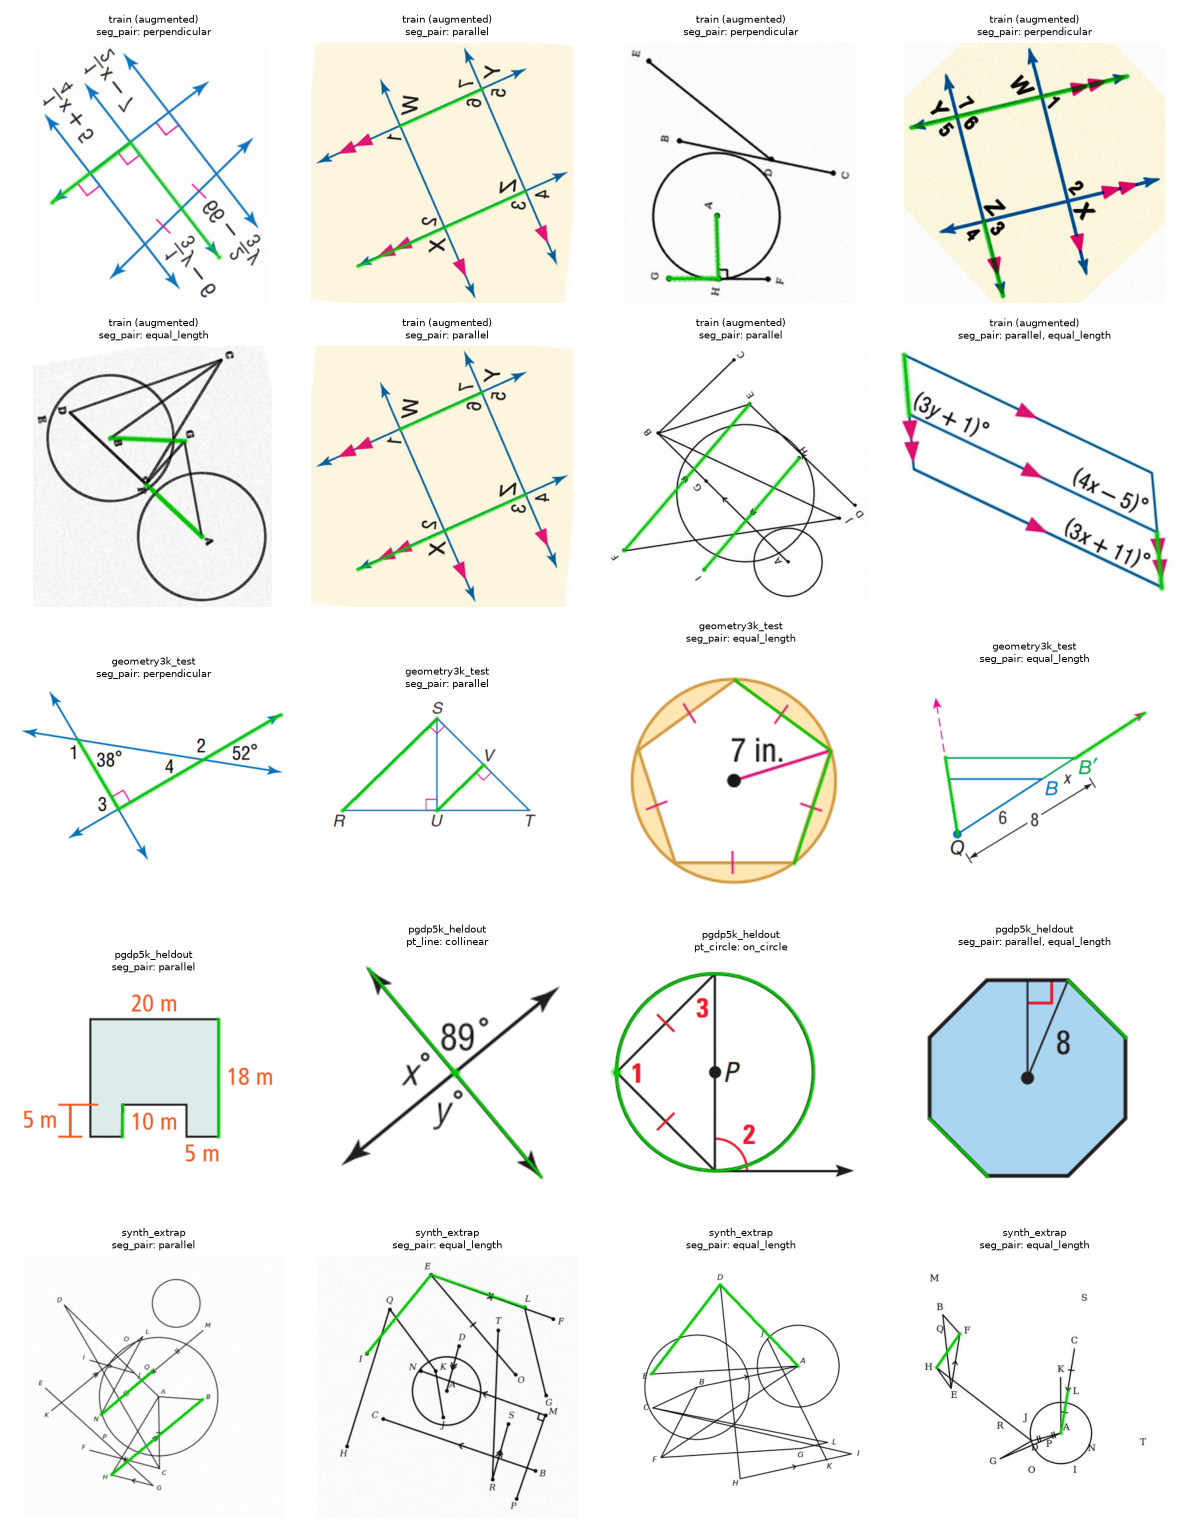
\includegraphics[width=\textwidth]{dataset_examples}
  \caption{Queries from each unit: augmented training queries (top two rows), in-distribution test, held-out source and synthetic extrapolation. The queried primitives are highlighted in green; everything else is the original image.}
  \label{fig:examples}
\end{figure}

\subsection{Inputs, targets and access}

The model input is one image and one query; the target is the six-way multi-label vector with its applicability mask, in two versions, \emph{asserted} and \emph{geometric}. Asserted positives in the training split, counted once per figure, are \nTrainParallel{} \rel{parallel}, \nTrainPerpendicular{} \rel{perpendicular}, \nTrainEqualLength{} \rel{equal\_length}, \nTrainOnCircle{} \rel{on\_circle}, \nTrainCollinear{} \rel{collinear} and \nTrainTangent{} \rel{tangent}; three further relation types available in the annotations (\rel{midpoint} \nTrainMidpoint, \rel{equal\_angle} \nTrainEqualAngle, \rel{perp\_bisector} \nTrainPerpBisector) fall below the pre-set inclusion threshold of \tierTwoMinPositives{} positives and are excluded. All three datasets are public under MIT licences through the authors' repositories or Hugging Face dataset cards, contain no personal data, and are small enough (under 10,000 distinct real diagrams, about 1 GB) to process on one machine; the archives are verified by SHA-256 on download.
